\documentclass[tikz, border=2pt]{standalone}
\usepackage{tikz}
\usepackage{amsmath}
\usetikzlibrary{arrows.meta,positioning,fit,backgrounds,calc,decorations.pathreplacing}
% Shared TikZ style, color-matched to paper/figures/*.pdf (matplotlib):
% ink = near-black strokes/fill, accent = deep red for the one thing per
% diagram that should draw the eye, grid = light gray for structure that
% should recede.
\definecolor{ink}{HTML}{1A1A1A}
\definecolor{accent}{HTML}{A6192E}
\definecolor{gridgray}{HTML}{D9D9D9}
\definecolor{panelbg}{HTML}{F2F2F2}

\tikzset{
  every node/.style={font=\sffamily},
  box/.style={draw=ink, thick, rounded corners=1.5pt, minimum height=0.75cm,
              font=\sffamily\small, align=center, fill=white, text=ink},
  stubbox/.style={box, draw=ink, dashed, fill=panelbg},
  hibox/.style={box, fill=ink, text=white},
  panel/.style={draw=none, fill=panelbg, rounded corners=2pt},
  arr/.style={-{Latex[length=2.2mm, width=1.6mm]}, thick, draw=ink},
  darr/.style={arr, dashed},
  accarr/.style={-{Latex[length=2.2mm, width=1.6mm]}, thick, draw=accent},
  lbl/.style={font=\sffamily\scriptsize, text=ink},
  ital/.style={font=\sffamily\itshape\scriptsize, text=ink!70},
  note/.style={font=\sffamily\scriptsize, align=left, text=ink},
  state/.style={draw=ink, thick, rounded corners=3pt, minimum width=2.6cm,
                minimum height=0.9cm, font=\sffamily\small, align=center, fill=white},
  finalstate/.style={state, fill=ink, text=white},
  abortstate/.style={state, draw=accent, thick, text=accent},
}

\tikzset{
  cell/.style={draw=ink, thick, minimum height=0.9cm, font=\sffamily\scriptsize, align=center, fill=white},
  hicell/.style={cell, fill=ink!8},
  brace/.style={decorate, decoration={brace, amplitude=4pt, raise=1pt}, thick, draw=ink!70},
}
\begin{document}
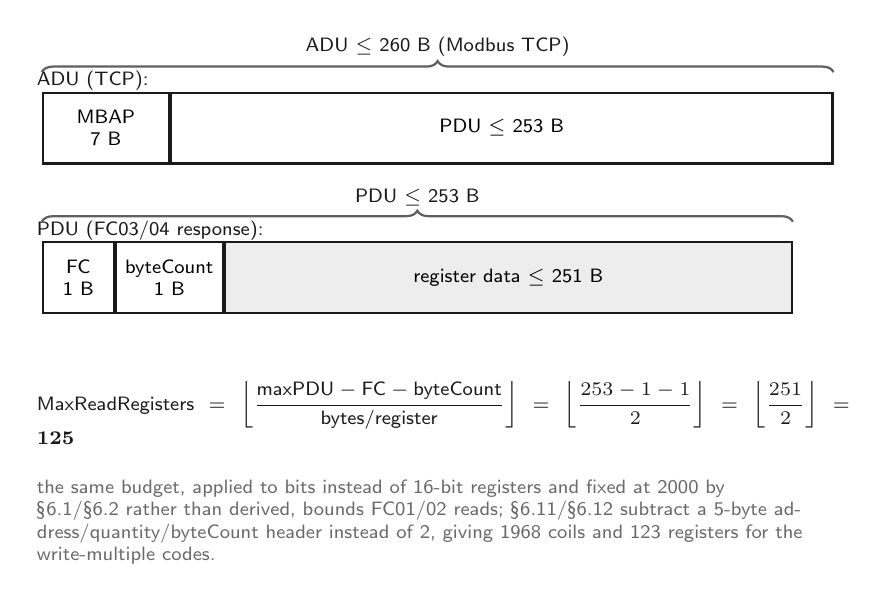
\begin{tikzpicture}

% --- Row 1: full ADU over TCP ---
\node[lbl, anchor=west] at (-0.2,3.4) {ADU (TCP):};
\node[cell, minimum width=1.6cm] (mbap) at (0.8+0,2.8) {MBAP\\7 B};
\node[cell, minimum width=8.4cm, anchor=west] (pdu1) at (mbap.east) {PDU \(\le\) 253 B};
\draw[brace] ([yshift=6pt]mbap.north west) -- ([yshift=6pt]pdu1.north east)
  node[midway, above=3pt, lbl] {ADU \(\le\) 260 B (Modbus TCP)};

% --- Row 2: PDU breakdown for a read-registers response ---
\node[lbl, anchor=west] at (-0.2,1.5) {PDU (FC03/04 response):};
\node[cell, minimum width=0.9cm] (fc) at (0.45,0.9) {FC\\1 B};
\node[cell, minimum width=0.9cm, anchor=west] (bc) at (fc.east) {byteCount\\1 B};
\node[hicell, minimum width=7.2cm, anchor=west] (data) at (bc.east) {register data \(\le\) 251 B};
\draw[brace] ([yshift=6pt]fc.north west) -- ([yshift=6pt]data.north east)
  node[midway, above=3pt, lbl] {PDU \(\le\) 253 B};

% --- Row 3: derivation ---
\node[note, text width=10.4cm, anchor=north west] at (-0.2,-0.3)
  {\(\text{MaxReadRegisters} \;=\; \left\lfloor \dfrac{\text{maxPDU} - \text{FC} - \text{byteCount}}{\text{bytes/register}} \right\rfloor \;=\; \left\lfloor \dfrac{253 - 1 - 1}{2} \right\rfloor \;=\; \left\lfloor \dfrac{251}{2} \right\rfloor \;=\; \mathbf{125}\)};
\node[note, text width=10.4cm, anchor=north west, text=ink!65] at (-0.2,-1.55)
  {the same budget, applied to bits instead of 16-bit registers and fixed at 2000 by \textsection6.1/\textsection6.2 rather than derived, bounds FC01/02 reads; \textsection6.11/\textsection6.12 subtract a 5-byte address/quantity/byteCount header instead of 2, giving 1968 coils and 123 registers for the write-multiple codes.};

\end{tikzpicture}
\end{document}
